\chapter{Desarrollo e implementación} % Main chapter title
\label{Chapter3} % Change X to a consecutive number; for referencing this chapter elsewhere, use \ref{ChapterX}

\definecolor{mygreen}{rgb}{0,0.6,0}
\definecolor{mygray}{rgb}{0.5,0.5,0.5}
\definecolor{mymauve}{rgb}{0.58,0,0.82}

%%%%%%%%%%%%%%%%%%%%%%%%%%%%%%%%%%%%%%%%%%%%%%%%%%%%%%%%%%%%%%%%%%%%%%%%%%%%%
% parámetros para configurar el formato del código en los entornos lstlisting
%%%%%%%%%%%%%%%%%%%%%%%%%%%%%%%%%%%%%%%%%%%%%%%%%%%%%%%%%%%%%%%%%%%%%%%%%%%%%
\lstset{ %
  backgroundcolor=\color{white},   % choose the background color; you must add \usepackage{color} or \usepackage{xcolor}
  basicstyle=\footnotesize,        % the size of the fonts that are used for the code
  breakatwhitespace=false,         % sets if automatic breaks should only happen at whitespace
  breaklines=true,                 % sets automatic line breaking
  captionpos=b,                    % sets the caption-position to bottom
  commentstyle=\color{mygreen},    % comment style
  deletekeywords={...},            % if you want to delete keywords from the given language
  %escapeinside={\%*}{*)},          % if you want to add LaTeX within your code
  %extendedchars=true,              % lets you use non-ASCII characters; for 8-bits encodings only, does not work with UTF-8
  %frame=single,	                % adds a frame around the code
  keepspaces=true,                 % keeps spaces in text, useful for keeping indentation of code (possibly needs columns=flexible)
  keywordstyle=\color{blue},       % keyword style
  language=[ANSI]C,                % the language of the code
  %otherkeywords={*,...},           % if you want to add more keywords to the set
  numbers=left,                    % where to put the line-numbers; possible values are (none, left, right)
  numbersep=5pt,                   % how far the line-numbers are from the code
  numberstyle=\tiny\color{mygray}, % the style that is used for the line-numbers
  rulecolor=\color{black},         % if not set, the frame-color may be changed on line-breaks within not-black text (e.g. comments (green here))
  showspaces=false,                % show spaces everywhere adding particular underscores; it overrides 'showstringspaces'
  showstringspaces=false,          % underline spaces within strings only
  showtabs=false,                  % show tabs within strings adding particular underscores
  stepnumber=1,                    % the step between two line-numbers. If it's 1, each line will be numbered
  stringstyle=\color{mymauve},     % string literal style
  tabsize=2,	                   % sets default tabsize to 2 spaces
  title=\lstname,                  % show the filename of files included with \lstinputlisting; also try caption instead of title
  morecomment=[s]{/*}{*/}
}

%----------------------------------------------------------------------------------------
% Resumen de capitulo
%----------------------------------------------------------------------------------------

En este capítulo se detallan los cambios fundamentales realizados sobre la estructura del código exitente, para portarlo a la EDU-CIAA-NXP y las mejoras introducidas. Además, se documenta, el desarrollo de los nuevos componentes de hardware virtuales, los ports de las bibliotecas y ejemplos de programa, así como nuevos programas.

%----------------------------------------------------------------------------------------
\section{Herramientas de desarrollo}
\label{sec:Herramientas de trabajo}
%----------------------------------------------------------------------------------------

En esta sección se exponen las herramientas del desarrollo que se utilizan en este trabajo.

%-------------------
\subsection{Plataforma de desarrollo EDU-CIAA-NXP}
\label{sec:EDU-CIAA-NXP}

La EDU-CIAA-NXP esta es la plataforma de hardware objetivo a emular del presente trabajo. Es uno de los diseños de hardware del Proyecto CIAA. En particular, el enfoque es ayudar a las Universidades Argentinas a migrar de microcontroladores de 8 bits a modernos microcontroladores de 32 bits al usar una placa diseñada en Argentina con hardware y software abiertos. Estas placas se difundieron en todas las universidades Argentinas con carreras de electrónica y afines, y también, en algunos países limítrofes. 
Se utilizó la placa física para ensayos de comparación entre lo real y el emulador web desarrollado.

%-------------------
\subsection{Editor \textit{VSCode}}
\label{sec:gitYAmigos}

Visual Studio Code \citep{VisualStudioCode}: es un editor de código fuente gratuito y de código abierto desarrollado por Microsoft. Incluye soporte para la depuración, control integrado de Git, resaltado de sintaxis, finalización inteligente de código, fragmentos, refactorización de código y muchas otras herramientas más. Se eligio este IDE, de la sigla en inglés Integrated Development Environment \citep{IDE}, por la capacidad de sus herramientas y la simpleza de su editor de código. El uso de este editor facilitó la escritura y el mantenimiento del código del emulador, mejorando la productividad y la calidad del desarrollo.
	
%---------------------------------------------
\subsection{Editor de gráficos vectoriales \textit{Inkscape}}
\label{sec:Inkscape}

Inkscape \citep{inkscape}: es un editor de gráficos vectoriales que permite crear, editar y modificar gráficos. En el proceso de desarrollo de la interfaz gráfica, se utilizó para diseñar diversos componentes de hardware.

%---------------------------------------------
\subsection{Sistemas de control de versiones e integración contínua}
\label{sec:gitYAmigos}

\begin{itemize}
	\item GitHub \citep{GitHub}: es una plataforma de desarrollo colaborativo que permite alojar proyectos utilizando el sistema de control de versiones Git. Se utilizó los servicios de esta plataforma para almacenar y
compartir el código fuente, de manera que se pueda hacer un seguimiento
de las últimas modificaciones realizadas.
	
	\item Travis CI \citep{TravisCI}: es un servicio de integración continua en la nube y es utilizado mayormente para configurar y ejecutar pruebas automatizadas en un entorno controlado y reproducible. Además, se integra con sistemas de control de versiones como GitHub y permite que con cada cambio realizado en el repositorio se ejecuten las pruebas definidas en el script de construcción.
De esta manera, se asegura la calidad del software. Incluso, proporciona informes detallados de las pruebas realizadas y servicio de notificaciones por correo electrónico.

	\item GitLab \citep{GitLab}: es una plataforma web de gestión de repositorios y permite la colaboración en el desarrollo de software. Proporciona un conjunto completo de herramientas para el ciclo de vida del desarrollo de software, por lo tanto, permite configurar pipelines de integración y entrega continua, en consecuencia, automatiza la compilación, las pruebas y el despliegue de software de manera eficiente. Es una alternativa a otras plataformas como GitHub con Travis CI.
\end{itemize}

%---------------------------------------------
\subsection{Herramientas de\textit{Testing}}
\label{sec:TestingFrontendBackend}

\textit{Arm Mbed OS Simulator} no posee ninguna plataforma de \textit{tests}. Los únicos tests encontrados pertenecen a la biblioteca \textit{Arm Mbed OS}, es por esto que se agregan las siguientes herramientas para \textit{testing} en el \textit{Frontend}:

\begin{itemize}
     \item Mocha \citep{Mocha}: es un marco de trabajo para pruebas de JavaScript que tiene funciones que se ejecutan en \textit{Node.JS} y en el navegador web. En consecuencia, hace que las pruebas asincrónicas sean simples. Asimismo, Las pruebas se ejecutan en serie y se realiza el envío de excepciones aún no detectadas a los casos de prueba correctos.
El uso de este marco de trabajo permite hacer pruebas sobre la interfaz de usuario de la plataforma.
     
     \item Chai \citep{Chai}: es una biblioteca de aserciones (como por ejemplo, \textit{assert}, \textit{expect} y \textit{should}) que puede usarse con cualquier marco de pruebas de Javascript. Chai se utiliza en las pruebas de \textit{EmuCIAA} para  verificar el comportamiento esperado de las funciones, componentes y datos generados. 
\end{itemize}

Mientras que para \textit{testing} en el \textit{Backend}, se agregan las siguientes:

\begin{itemize}
    \item \textit{Check} \citep{Check}: es una biblioteca de pruebas unitarias para el lenguaje de programación C que proporciona un conjunto de macros y funciones que facilitan la escritura y la ejecución de las pruebas unitarias. Además, provee mecanismos que aislan y ejecutan las pruebas en un entorno controlado y separado, usando suites de pruebas, funciones de inicialización y limpieza. Se utilizó en \textit{EmuCIAA} para verificar el correcto funcionamiento de las funciones y componentes implementados en el backend escritos en lenguaje C.
    
    \item \textit{CMocka} \citep{CMocka}: es una biblioteca de pruebas unitarias especialmente diseñada para C, destacandose por su capacidad de crear \textit{mocks} (falsos) y \textit{stubs} (simulaciones) de funciones. De esta manera se logra probar componentes de código que dependen de funciones externas. Y, además, facilita el aislamiento de las unidades de código y la creación de escenarios de prueba que pueden ser controlados. El uso de esta tecnología permite simular funciones mediante \textit{mocks} para controlar el comportamiento de las funciones dependientes y facilitar las pruebas de código que interactúa con dichas funciones.
\end{itemize}

En el capítulo \ref{Chapter4} se muestran estas herramientas en uso.

%---------------------------------------------
\subsection{Servidor en la nube \textit{DigitalOcean}}
\label{sec:DigitalOcean}

\textit{DigitalOcean} \citep{DigitalOcean}: ofrece servicios de infraestructura de computación en la nube, tales como permitir a los usuarios crear y administrar servidores virtuales, conocidos como Droplets. Incluso, ofrece opciones de almacenamiento, configuración de redes privadas virtuales, servicios de bases de datos, entre otros. DigitalOcean se destaca por su enfoque en la simplicidad y la facilidad de uso de su plataforma. El emulador desarrollado en el presente trabajo se encuentra desplegado en el servidor de DigitalOcean.


%----------------------------------------------------------------------------------------
\section{Restructuración de archivos y carpetas}
%----------------------------------------------------------------------------------------

Luego de comprender el funcionamiento de \textit{Arm Mbed OS Simulator}, se comienza el desarrollo de este trabajo. Se utiliza a partir de aquí el nombre \textit{EmuCIAA}, para referirse al \textit{Emulador de la placa EDU-CIAA-NXP}.

En principio, se eliminaron módulos y dependencias innecesarias para el alcance de este trabajo, tales como: \textit{mbed-http}, \textit{simple-mbed-cloud-client}, \textit{features}, \textit{rtos} y todas las sub-carpetas dentro de la carpeta \textit{target} excluyendo la sub-carpeta TARGET\_SIMULATOR. Se modificaron las carpetas y archivos de configuración para adaptarlos al desarrollo del entorno del emulador para la placa EDU-CIAA-NXP. Luego, se reemplazó \textquotedbl mbed-os\textquotedbl{}  por la biblioteca \textit{\textbf{sAPI}}, pero se mantuvieron algunos componentes propios de Mbed, como \textit{events} y \textit{callback}, para agilizar el desarrollo.

La figura \ref{fig:estructuraCiaa}, exhibe la nueva estructura de carpetas y archivos realizada para \textit{EmuCIAA}.

\begin{figure}[ht]
	\centering
	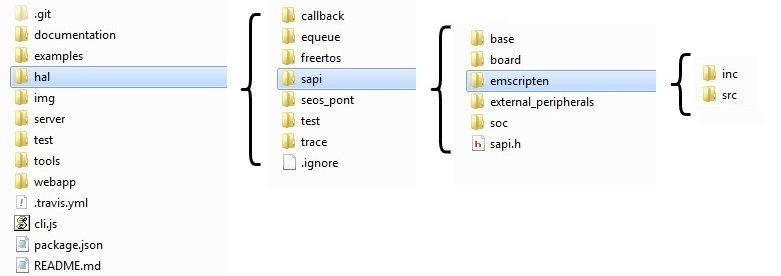
\includegraphics[scale=.55]{./Figures/estructuraCiaa.jpg}
	\caption{Estructura de carpetas y archivos de \textit{EmuCIAA}.}
	\label{fig:estructuraCiaa}
\end{figure}

En las siguientes secciones se detallan todos estos cambios y agregados relizados.

%----------------------------------------------------------------------------------------
\section{\textit{Frontend}: rediseño de la Interfaz de Usuario}
%----------------------------------------------------------------------------------------

Para el rediseño de la interfaz, se optó por un diseño intuitivo, de manera que el usuario se sienta familiarizado con las herramientas de trabajo y que la disposición de los componentes sea cómoda y esté organizada al momento de usarlas, reordenando los elementos en pantalla.

Para su estudio, la figura \ref{fig:PlataformaEmulador1} muestra la interfaz gráfica de \textit{EmuCIAA}dividida en tres partes.

\begin{figure}[ht]
	\centering
	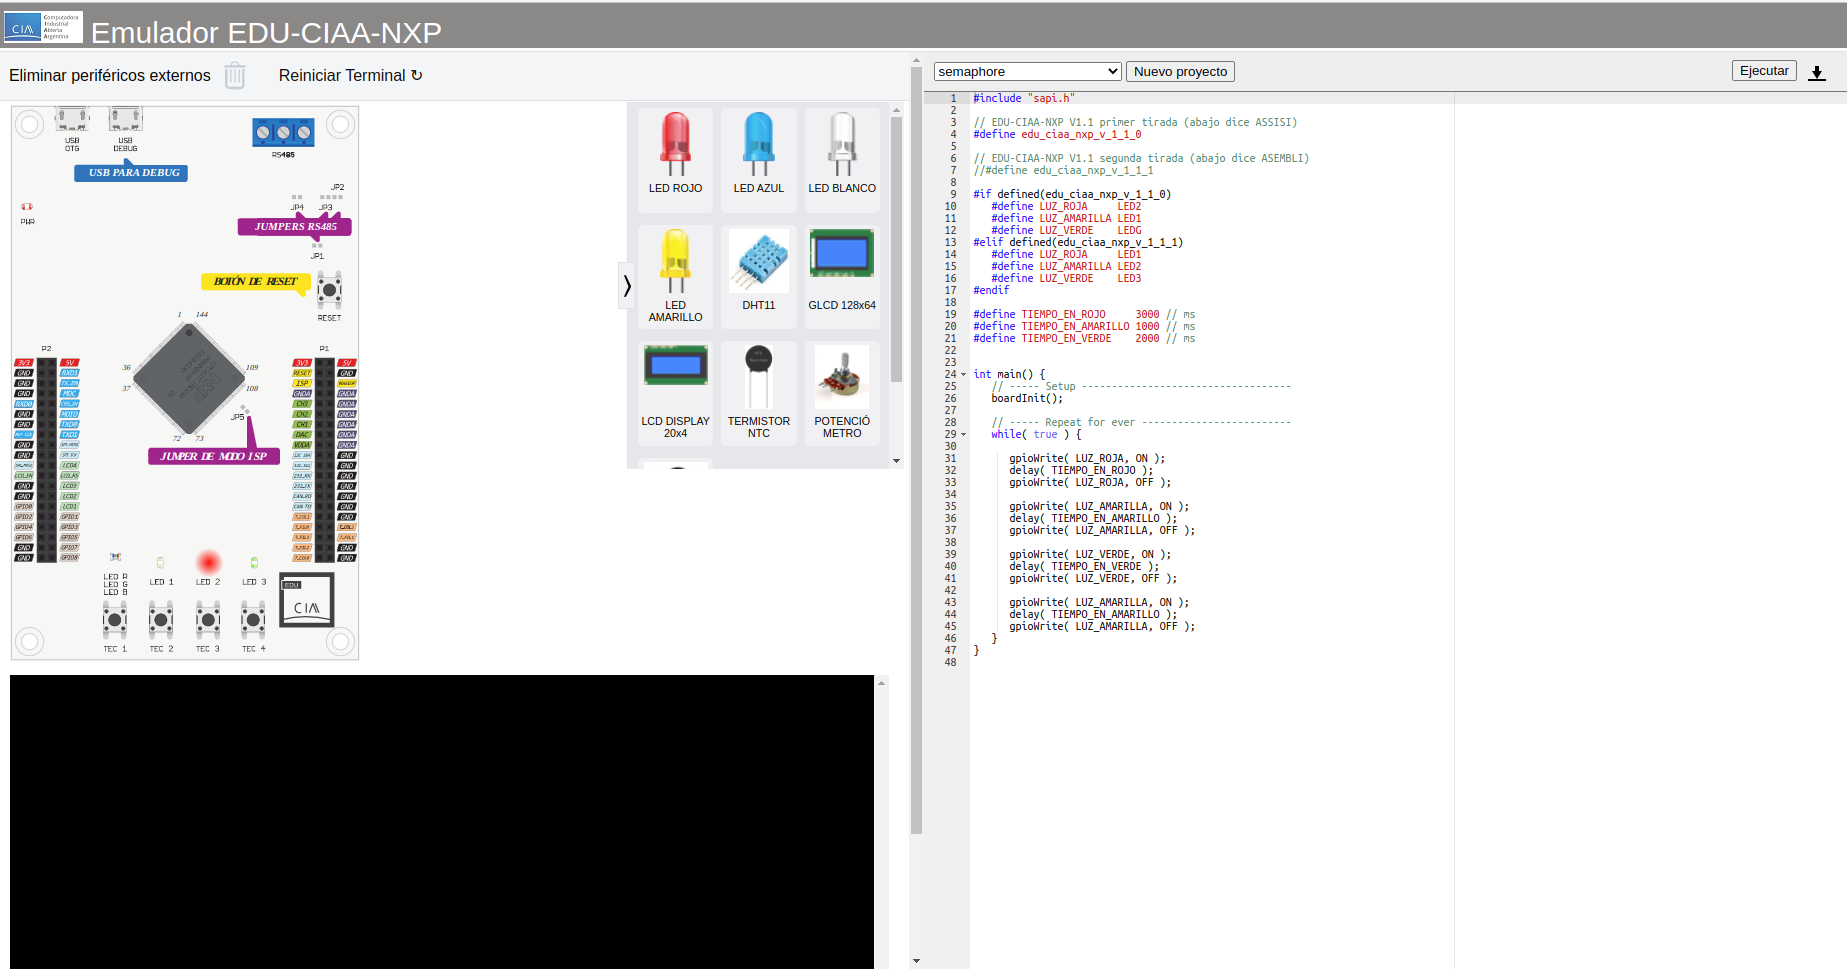
\includegraphics[scale=.28]{./Figures/PlataformaEmulador.png}
	\caption{Interfaz gráfica de \textit{EmuCIAA}.}
	\label{fig:PlataformaEmulador1}
\end{figure}

Por consiguiente, el diseño de la interfaz de usuario de la plataforma proporciona las siguientes áreas:

\begin{itemize}
	\item Área de ensamblado: el valor predeterminado muestra la placa EDU-CIAA-NXP, y también se permite agregar componentes externos.
	\item Área de codificación: se proporciona un editor de código en línea para programar con la placa EDU-CIAA-NXP. La primera vez que se accede a la platafoma se muestra en ejecución un ejemplo de código predeterminado (ejemplo \textit{blinky.c}). Se mantuvo \textit{Ace} como editor.
	\item Área de consola integrada: se muestra en una ventana la salida de las UARTs de la EDU-CIAA-NXP. Se reutilizó \textit{xterm} para la consola.
\end{itemize}

Dadas las áreas de trabajo que presenta la plataforma, el usuario programador podrá realizar las siguientes tareas:

\begin{itemize}
	\item Probar los programas de ejemplo predeterminados.
	\item Crear un nuevo programa desde cero, o bien, modificar un ejemplo.
	\item Editar y ejecutar programas.
	\item Visualizar los cambios programados en la placa virtual.
	\item Agregar componentes de hardware virtual para conectar a la placa virtual.
	\item Ver los errores obtenidos en la programación.
	\item Ver la salida de las UARTs de la placa virtual.
\end{itemize}

%--------------------------------------
\subsection{Área de ensamblado}

Para el desarrollo de la placa EDU-CIAA-NXP, y componentes externos para conectar a la misma, se agregaron los gráficos SVG (SVG) por las siguientes características:

\begin{itemize}
	\item Son más ligeras, entonces se cargan más rápido en el navegador.
    \item Por su capacidad de ser modificado por medio de \textit{JavaScript}. Por lo tanto, se pudieron crear imágenes interactivas.
	\item Evitan que las imagenes se deformen y no pierden calidad.
	\item Permite programar animaciones.
\end{itemize}

Estos gáficos fueron proporcionados por el co-director del presente trabajo, Mg. Ing. Eric Pernia:

\begin{itemize}
    \item SVG EDU-CIAA-NXP \citep{SVGFirmwareV3}.
    \item SVG LED.
    \item SVG DHT11.
    \item SVG Potenciómetro \(10K\Omega\).
    \item SVG Termistor NTC. 
    \item SVG Analog Stick. 
    \item SVG Display LCD 20x4 caracteres.
    \item SVG Display GLCD 128x64 píxeles y 16x4 caracteres.
\end{itemize}

Estos componenetes se combinan con a elementos de \textit{JavaScript}, para brindar a los usuarios una experiencia visual interactiva. Asimismo, se incorporaron fuentes tipográficas en los dibujos SVG para las representaciones de texto. Estas fuentes están definidas en información vectorial, lo que permitió una visualización nítida y escalable en diferentes tamaños para las pantallas LCD y GLCD.

En la capa de programación \textit{JS UI}, se implementa el comportamiento interactivo para los botones de la placa (TEC1, TEC2, TEC3 y TEC4), los cuales permiten ser pulsados; y los LEDs (LED\_RGB, LED1, LED2 y LED3), que permiten mostrar los estados de encendido y apagado en la placa virtual.

En \textit{Arm Mbed OS Simulator}, para agregar componentes y conectarlos a la placa de desarrollo, existe botón que muestra la lista de componentes disponibles en una ventana. Con el objetivo de optimizar la experiencia del usuario, se desarrollo para \textit{EmuCIAA} un nuevo \textit{sidebar} (barra lateral) colapsable, donde se exhiben todos componentes. De esta manera, para agregar un componente, el usuario debe expandir la barra lateral y hacer \textit{click} sobre el perifperico elegido. Al realizar esta acción aparece una ventana modal para realizar la configuración de las conexiones entre el componente y la EDU-CIAA-NXPl (figura \ref{fig:AgregarPeriferico}). 

\begin{figure}[ht]
	\centering
	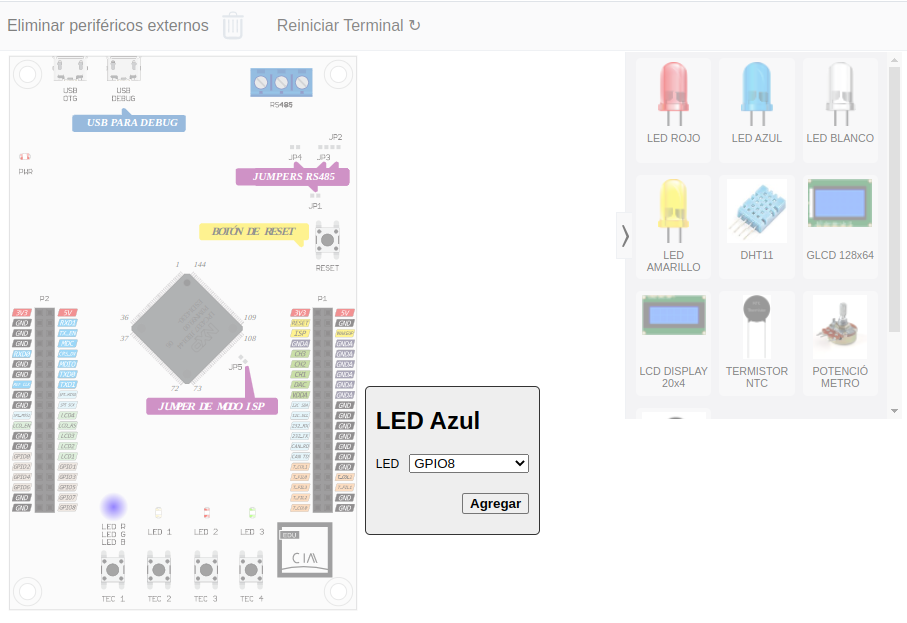
\includegraphics[scale=.37]{./Figures/AgregarPeriferico.png}
	\caption{El usuario puede elegir un componente en la aplicación.}
	\label{fig:AgregarPeriferico}
\end{figure}

\newpage

Una vez aceptada la configuración, la barra automáticamente colapsa, ocultándose del área de ensamblado. Al colapsarse, se muestra el periférico integrado en la aplicación (figura \ref{fig:AgregarPeriferico2}). 

\begin{figure}[ht]
	\centering
	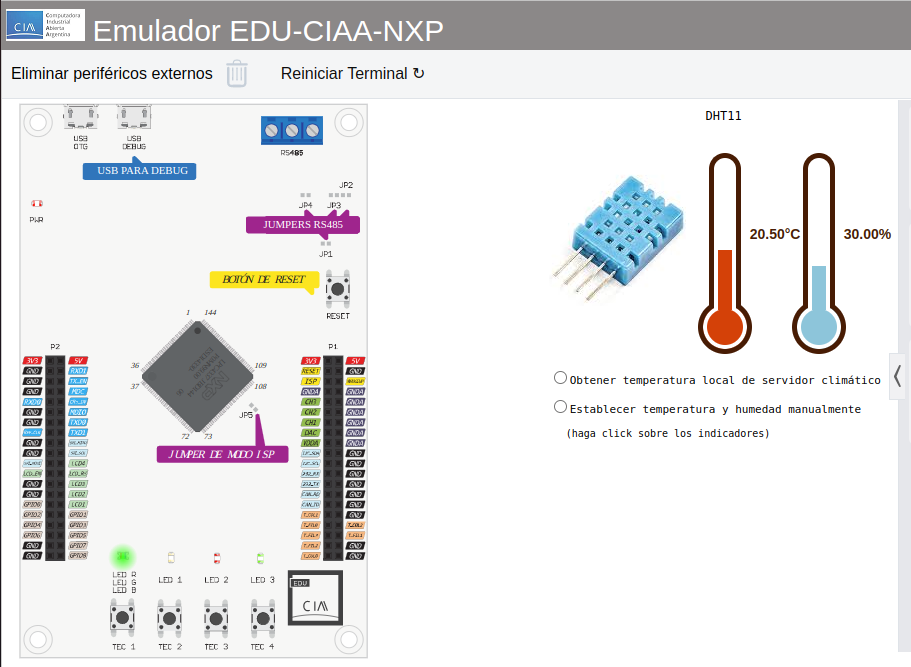
\includegraphics[scale=.37]{./Figures/AgregarPeriferico2.png}
	\caption{Periférico agregado en el área de ensamblado. }
	\label{fig:AgregarPeriferico2}
\end{figure}

Para eliminar un componente, simplemente debe seleccionar el componente deseado, y se habilita el icono de \textquotedbl Eliminar periféricos externos\textquotedbl. Al hacer clic en el icono, el periférico virtual es eliminado de la pantalla.

%-----------------------------------------
\subsection{Área de codificación}

Esta parte de la plataforma se reserva al usuario para que pueda programar sus aplicaciones. Esta ventana de edición presenta las siguientes capacidades:

\begin{itemize}
\item Manejar la sintaxis para los lenguajes C/C++. Esto significa que permite el uso de las palabras claves, comentarios, constantes, etc., realizando el coloreo de sintaxis.
\item Resaltado de líneas de código, sangría automática y número de línea.
\item Función buscar (ctrl + f).
\item Función buscar/reemplazar (ctrl + h).
\item Función deshacer (ctrl + z).
\item Función rehacer (ctrl + y).
\end{itemize}

Para compilar un programa, la plataforma provee al usuario el botón “Ejecutar”. Si existen errores en el código, que no permitan la compilación, se muestran los mismos en pantalla. Como ejemplo, en la figura \ref{fig:PlataformaErrores2} se muestra un código que genera los errores de compilación. Mientras que en la figura \ref{fig:PlataformaErrores1} se presentan los errores de compilación que se muestran en el área de ensamblado en dicho caso luego de intentar ejecutar el programa.

\begin{figure}[ht]
	\centering
	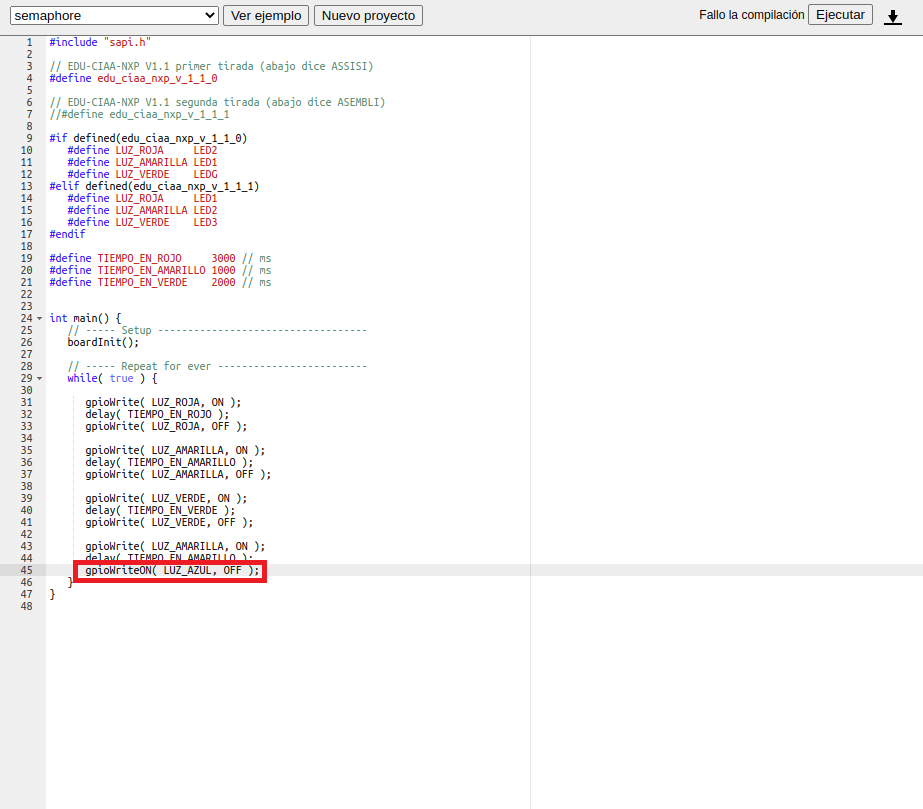
\includegraphics[scale=.42]{./Figures/PlataformaErrores1.png}
	\caption{Código que genera errores de compilación.}
	\label{fig:PlataformaErrores2}
\end{figure}

\begin{figure}[ht]
	\centering
	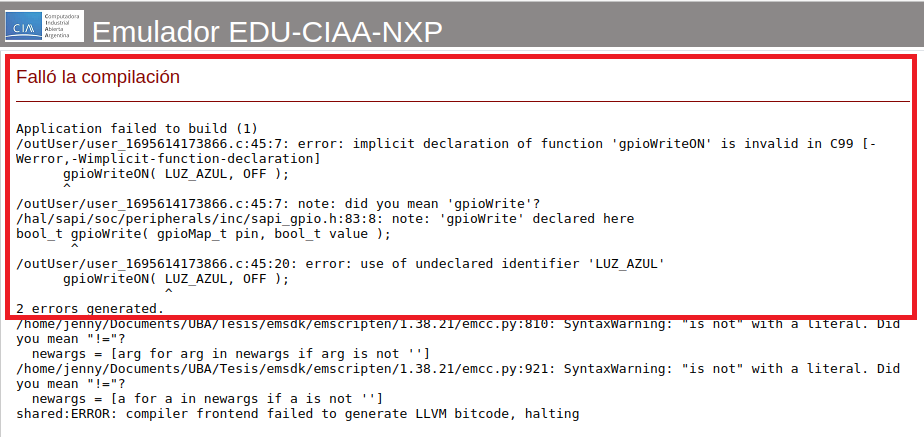
\includegraphics[scale=.39]{./Figures/PlataformaErrores2.png}
	\caption{Errores de compilación.}
	\label{fig:PlataformaErrores1}
\end{figure}

\hfill \break

También, se implementó una estructura jerárquica en la lista desplegable de ejemplos. El propósito es organizar y presentar los ejemplos agrupados por periféricos, de manera más ordenada y fácil de navegar para el usuario. La figura \ref{fig:listExamples} muestra la estructura jerárquica de la lista de ejemplos.

\begin{figure}[ht]
	\centering
	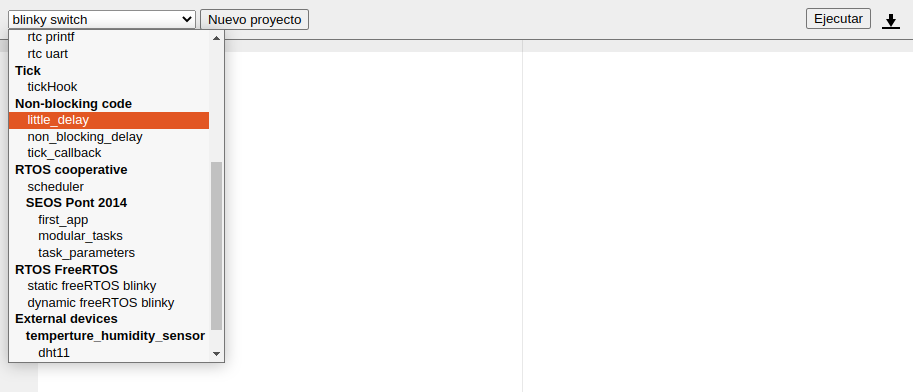
\includegraphics[scale=.42]{./Figures/listExamples.jpg}
	\caption{Estructura jerárquica de ejemplos. }
	\label{fig:listExamples}
\end{figure}

Ademas, la aplicación automáticamente carga dentro del área de ensamblado un periférico con las conexiones a los pines configurados por defecto, cuando el usuario selecciona algún ejemplo que contenga un periférico externo, De esta manera, el usuario ya no tiene la necesidad de seleccionar y configurar el periférico para probar un ejemplo. La figura \ref{fig:cargarPeriferico} muestra el periférico agregado automáticamente al seleccionar el ejemplo \textquotedbl potentiometer\textquotedbl.

\begin{figure}[ht]
	\centering
	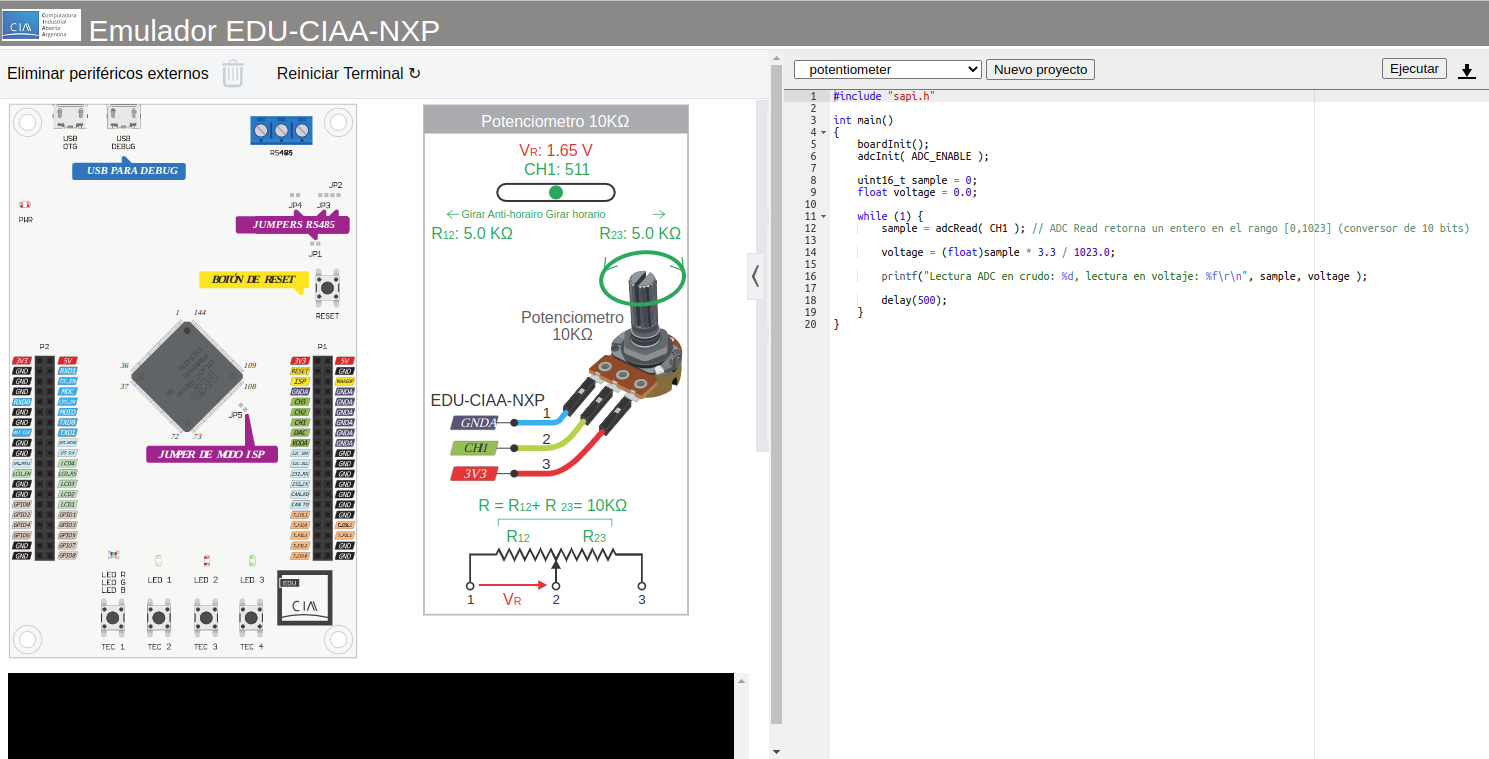
\includegraphics[scale=.31]{./Figures/cargarPeriferico.png}
	\caption{Carga automática del periférico. }
	\label{fig:cargarPeriferico}
\end{figure}

%------------------------------------------
\subsection{Área de consola integrada}

Dentro del código traducido en el proceso de compilación por \textit{Emscripten}, se encuentran las siguientes funciones definidas y configuradas previamente: 

\begin{itemize}
\item \texttt{print}, esta función envía el texto a la terminal de la interfaz gráfica del emulador web, al utilizar la función \texttt{terminal.write}.
\item \texttt{printErr}, se comunica con la consola de error del navegador, al usar \newline \texttt{console.error}.
\end{itemize}

Ambas funciones interactuan con el código \textit{JavaScript}. La función \texttt{printErr} se comunica con la consola de error del navegador y la función \texttt{print} se comunica con la terminal de \textit{EmuCIAA} a través de la biblioteca \textit{xterm.js}.

Entre las principales características de \textit{xterm.js} se destaca:

\begin{itemize}
    \item Funciona con la mayoría de las aplicaciones de terminal, como por ejemplo, bash, siendo compatible con aplicaciones basadas y eventos de mouse.
    \item Es de alto rendimiento, por eso es realmente rápido.
    \item No requiere de dependencias externas para funcionar. La dependencia principal para el funcionamiento básico es el propio navegador web.
    \item API bien documentada.
\end{itemize}

Además de las características destacadas, \textit{xterm.js} es una biblioteca que fue adoptada por diversos proyectos populares, tales como VS Code, Hyper y Theia. La amplia adopción de \textit{xterm.js} por parte de estos proyectos contribuyo a la expansión de su comunidad de desarrolladores, quienes brindan un sólido respaldo y soporte.

En la figura \ref{fig:Terminal1} se muestra un programa de ejemplo que genera imprime por consola y en la figura \ref{fig:Terminal2} se puede observar dicha salida reflejada.

\begin{figure}[ht]
	\centering
	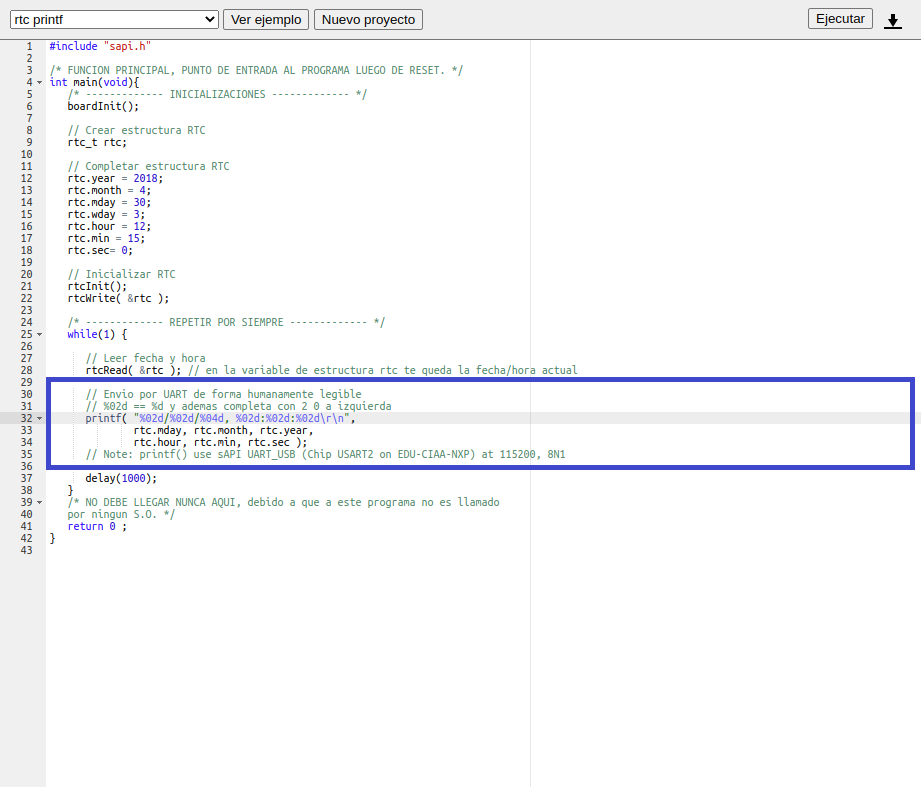
\includegraphics[scale=.70]{./Figures/Terminal1.png}
	\caption{Programa de usuario que imprime por consola.}
	\label{fig:Terminal1}
\end{figure}

\begin{figure}[ht]
	\centering
	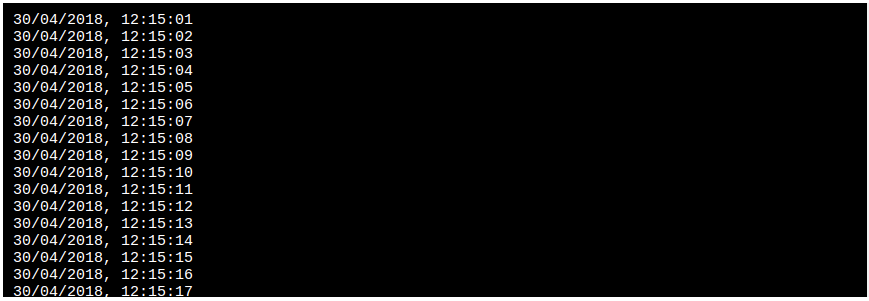
\includegraphics[scale=.70]{./Figures/Terminal2.png}
	\caption{Salida de la terminal serie.}
	\label{fig:Terminal2}
\end{figure}


%----------------------------------------------------------------------------------------
\section{\textit{Backend}: bibliotecas de C portadas}
\label{sec:BibC}
%----------------------------------------------------------------------------------------

A continuación se describen las principales bibliotecas de C portadas a \textit{EmuCIAA}, las cuales fueron extraídas del repositorio \textit{firmware\_v3} del Proyecto CIAA, descargando la última release estable al momento de comenzar este proyecto. Esta release corresponde a la versión \textit{r1.3.0} \citep{firmwareV3r130}:

\begin{itemize}
    \item \textit{sAPI} \citep{sAPICIAA}: esta biblioteca escrita en lenguaje C y compatible con C++ implementa una API simple que funciona como una capa de abstracción de hardware para microcontroladores. Es la principal biblioteca del Proyecto CIAA para el desarrollo de aplicaciones en C/C++ en los \textit{frameworks Firmware v2} \citep{firmwareV2} y \textit{Firmware v3}. 
    \item \textit{seos\_pont} \citep{seospont}: es un sistema operativo de tiempo real para microcontroladores, de código abierto, muy sencillo que permite definir tareas que se ejecutan en forma cooperativa, periódicamente. 
    \item \textit{freeRTOS}: \citep{freeRTOS} FreeRTOS es un sistema operativo de tiempo real para microcontroladores, de código abierto, que facilita la programación, el despliegue, la protección, la conexión y la administración de dispositivos periféricos pequeños y de bajo consumo. Permite trabajar en modo de ejecuciópn de tareas apropiativo o cooperativo.
\end{itemize}

En las siguientes secciones se describen los detalles más sobresalientes de la implementación realizada para llevar a cabo estos \textit{ports}.

%----------------------------------------------------------------------------------------
\section{Biblioteca \textit{sAPI}}
\label{sec:sAPI}
%----------------------------------------------------------------------------------------

Para la emulación a nivel de API, se implementa el \textit{port} de la biblioteca \textit{sAPI v0.6.2} para que funcione en la web, en lugar de funcionar en el hardware de un microcontrolador real. De esta manera, se proporciona una interfaz idéntica, permitiendo a los usuarios del emulador, programar en la plataforma web de la misma manera que lo harían con la placa EDU-CIAA-NXP real, logrando que cualquier programa escrito utilizando la sAPI pueda correr en el emulador.

Cabe destacar que al emular a nivel de sAPI, el usuario no podrá utilizar funciones de bajo nivel de la EDU-CIAA-NXP, como ser la biblioteca del fabricante del microcontrolador (LPCopen\citep{lpcopen}), o el acceso directo a registros físicos del microcontrolador, al igual que sucede con el emulador \textit{Arm Mbed OS Simulator}.

Para llevar a cabo la tarea de portar la sAPI a \textit{EmuCIAA}, se identificaron las funciones originales. Luego, en \textit{EmuCIAA} se han creado interfaces que reflejan su composición, que incluye definiciones de funciones, estructuras de datos y constantes.
De esta manera, en las funciones originales se examinaron los parámetros de entrada y los valores de retorno, para luego mapearlos correctamente en las definiciones de las funciones de \textit{EmuCIAA}. 

Asimismo, se utiliza un esquema de nomenclatura de los archivos de encabezado y de código fuente igual al de las bibliotecas originales. Esto permite mantener una estructura organizada y coherente en la emulación, que facilita el mantenimiento y comprensión.

Se reutilizó el archivo de encabezado \texttt{sapi.h} que cumple con la misma funcionalidad que en la biblioteca \textit{\textbf{sAPI}}, la cual consiste en incluir todos los módulos que conforman la biblioteca para utilizar en el programa de usuario. 

También se reutilizaron los archivos de encabezado: \texttt{sapi\_datatypes.h} y \newline \texttt{sapi\_peripheral\_map.h} incluidos en todos los módulos de la biblioteca \textit{\textbf{sAPI}} para permitir el uso de los tipos de datos básicos y nombres de periféricos de la placa. En la tabla \ref{tab:ConfiguracionGPIO} se muestran los tipos de datos de \texttt{sapi\_peripheral\_map.h} que se usan para los pines GPIO en la plataforma de emulación. 

\begin{table}[h]
	\centering
	\caption[\texttt{sapi\_peripheral\_map.h}.]{Tipos de datos de \texttt{sapi\_peripheral\_map.h} que se reutilizan en en la plataforma de emulación.}
	\begin{tabular}{l c c c}    
		\toprule
		\textbf{P2 header} & \textbf{P1 header} & \textbf{LEDs}  & \textbf{Switches}\\
		\midrule
		GPIO8, GPIO7, GPIO5 & T\_FIL1 &  LEDR &  TEC1\\		
		GPIO3, GPIO1, LCD1 & T\_COL2  & LEDG &  TEC2\\
		LCD2, LCD3, LCDRS & T\_COL0 & LEDB &  TEC3\\
		LCD4, SPI\_MISO, ENET\_TXD1 & T\_FIL2 & LED1 & TEC4\\
		ENET\_TXD0, ENET\_MDIO, ENET\_CRS\_DV & T\_FIL3 & LED2 & \\
	    ENET\_MDC, ENET\_TXEN, ENET\_RXD1 & T\_FIL0 & LED3 & \\
	    GPIO6, GPIO4, GPIO2 & T\_COL1&  & \\
	    GPIO0, LCDEN, SPI\_MOSI, ENET\_RXD0 & CAN\_TD&  & \\
		\bottomrule
		\hline
	\end{tabular}
	\label{tab:ConfiguracionGPIO}
\end{table}

Se puede observar que se reutilizó los nombres: TEC1, TEC2, TEC3 y TEC4 para los botones y los nombres LEDR, LEDG, LEDB, LED1, LED2 y LED3 para los LEDs de la placa EDU-CIAA-NXP.

Se realizó el \textit{port} de los siguientes módulos de la biblioteca \textit{sAPI}:

\begin{itemize}
    \item \textit{sapi\_board}: Contiene funciones de inicialización para la plataforma de hardware.
    \item \textit{sapi\_gpio}: Es una \textit{HAL} para pines E/S de porpósito general (en inglés, \textit{GPIO}).
    \item \textit{sapi\_uart}: Es una \textit{HAL} para periféricos \textit{UART}.
    \item \textit{sapi\_adc}: Es una \textit{HAL} para conversores a Analógico-Digital \textit{ADC}.
    \item \textit{sapi\_rtc}: Es una \textit{HAL} para el periférico rejoj de tiempo real, \textit{RTC}.
    \item \textit{sapi\_tick}: Es una \textit{HAL} que permite programar interrupciones períodicas.
    \item \textit{sapi\_delay}: Implementa funciones de retardos bloqueantes y no bloqueantes.
    \item \textit{sapi\_dht11}: Implementa un driver para el sensor de Humedad y temperatura DHT11.
    \item \textit{sapi\_display}: Implementa un driver para displays LCD y GLCD.
\end{itemize}

Existen otros módulos de \textit{sAPI} independientes del hardware como, por ejemplo, \textit{sapi\_button}, los cuales son independientes del hardware y se utilizaron para los ejemplos de en este trabajo sin modificaciones. El resto de los módulos que implementan otros periféricos, como por ejemplo \textit{I2C}, se dejan como trabajo a futuro.

En las siguientes secciones se muestran destalles de implementación de algunos de los módulos \textit{portados}.

%---------------------------------------------
\subsection{\textit{\textbf{sapi\_gpio}}}

Para comenzar a emular la biblioteca \textit{sapi\_gpio} del proyecto CIAA, se identificaron las funciones principales que el entorno de la plataforma web debería ofrecer al usuario. La siguiente tabla \ref{tab:sapiGPIO} muestra las funciones del archivo de código fuente \textit{sapi\_gpio} en la biblioteca \textit{\textbf{sAPI}}, que incluye los nombres de la funciones, los tipos de parámetros y el tipo de valor de retorno. Cabe destacar que estas definiciones son idénticas tanto en las \textit{\textbf{sAPI}} como en \textit{EmuCIAA}, lo que permite una correspondencia directa entre ambas.

\begin{table}[h]
	\centering
	\caption[Funciones \texttt{sapi\_gpio}]{Funciones \texttt{sapi\_gpio}}
	\begin{tabular}{p{0.20\linewidth} p{0.50\linewidth}  p{0.20\linewidth}}    
		\toprule
		\textbf{Función} 	 & \textbf{Parámetros} 		& \textbf{Tipo de retorno}  \\
		\midrule
		gpioInit & gpioMap\_t pin, gpioInit\_t config 		&  bool\_t \\		
		gpioRead	 & gpioMap\_t pin			&  bool\_t \\
		gpioWrite	 & gpioMap\_t pin, bool\_t value			& bool\_t \\
		gpioToggle	 & gpioMap\_t pin				&  bool\_t \\
		\bottomrule
		\hline
	\end{tabular}
	\label{tab:sapiGPIO}
\end{table}

Al igual que en la biblioteca \textit{\textbf{sAPI}} del proyecto CIAA, los archivos de código fuente para la plataforma de emulación, conservan el mismo nombre, por ejemplo  \texttt{sapi\_gpio.c}. Sin embargo, la implementación de las funciones es totalmente distinta. En el caso de la biblioteca \textit{\textbf{sAPI}} del proyecto CIAA, para \texttt{sapi\_gpio.c}  se incluyen los archivos de encabezado: \texttt{gpio\_18xx\_43xx.h} y \newline \texttt{scu\_18xx\_43xx.h}. Y en el caso de la plataforma de emulación se usa otro archivos de encabezado como \texttt{gpio\_api.h} para replicar el mismo comportamiento.

A continuación, se presenta una comparación entre las dependencias del módulo GPIO de la biblioteca \textit{\textbf{sAPI}} del proyecto CIAA (figura \ref{fig:GPIOsAPI}) y el módulo GPIO implementado en \textit{EmuCIAA} (figura \ref{fig:GPIOEmulador}). 

\begin{figure}[ht]
	\centering
	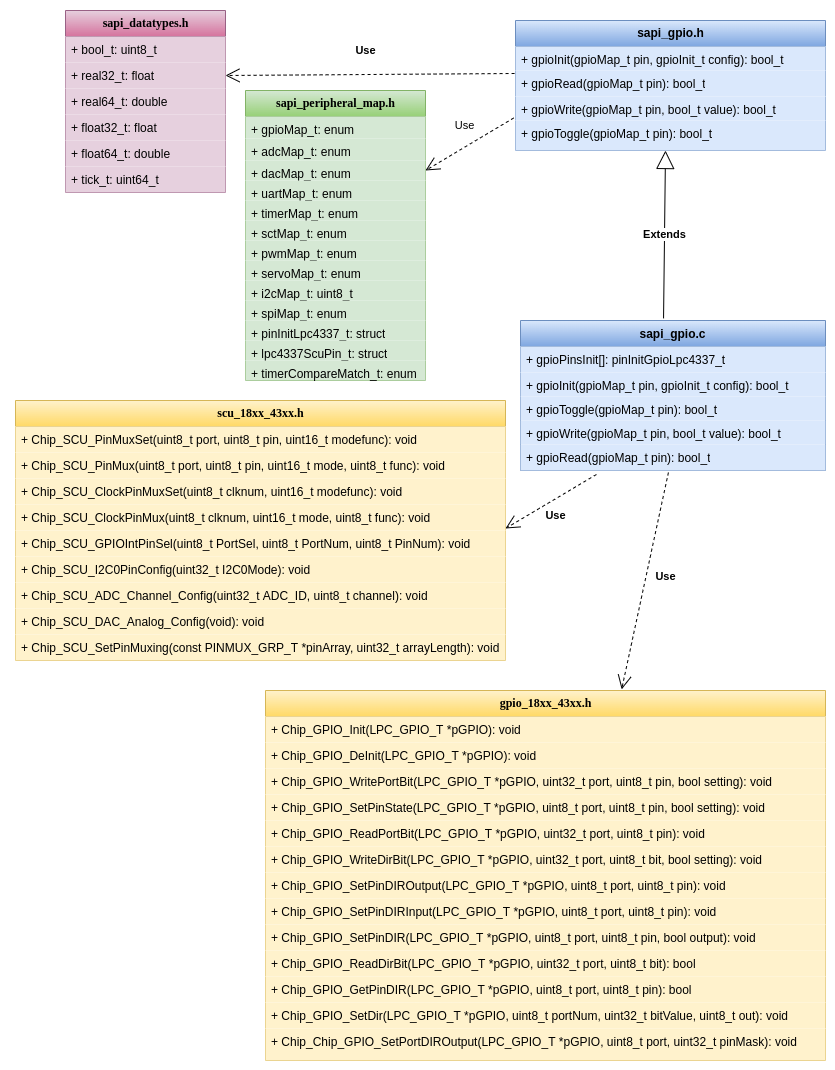
\includegraphics[scale=.50]{./Figures/DiagramaClasesGPIOsAPI.png}
	\caption{Dependencias del módulo \textit{GPIO} de la \textit{sAPI}}
	\label{fig:GPIOsAPI}
\end{figure}

\begin{figure}[ht]
	\centering
	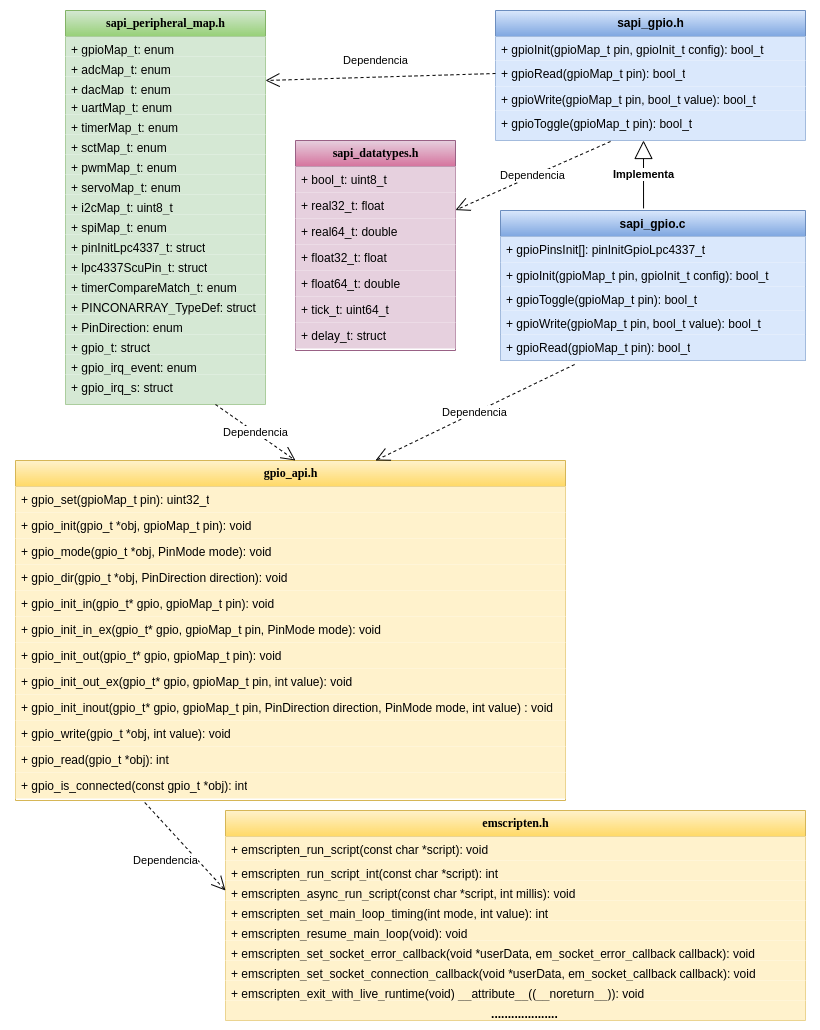
\includegraphics[scale=.46]{./Figures/DiagramaClasesEmulador.png}
	\caption{Dependencias del módulo \textit{GPIO} de \textit{EmuCIAA}.}
	\label{fig:GPIOEmulador}
\end{figure}

\newpage

Para lograr replicar el comportamiento de cada función, de manera que al invocarlas produzcan los mismos resultados sque se obtendrían al utilizar las funciones con el hardware físico, se utiliza la \textit{API} de \textit{Emscripten} en la capa de \textit{C HAL} para emular las siguientes funcionalidades:

\begin{itemize}
	\item \texttt{Chip\_GPIO\_Init(LPC\_GPIO\_PORT)} se utiliza para inicializar y configurar el hardware de los pines GPIO de la placa. En la capa de emulación \textit{C HAL} se realizaron configuraciones de variables para representar los tipos de pines e inicializarlos.
	
	\item \texttt{Chip\_GPIO\_SetDir (LPC\_GPIO\_PORT, gpioPort, \newline (1 \<<\<<  gpioPin), GPIO\_OUTPUT)} se utiliza para establecer la dirección de un pin, es decir, si se utilizará como entrada o salida. Se implementaron configuraciones similares para la capa \textit{JS HAL} usando las macros de \textit{Emscripten}.
	
	\item \texttt{Chip\_GPIO\_SetPinState(LPC\_GPIO\_PORT, gpioPort, \newline gpioPin, 0)} se utiliza para establecer el estado de los pines configurados como salida y establecer su valor lógico (alto o bajo). En la capa de abstracción de datos \textit{C}, esta función actualiza la estructura de datos utilizada para almacenar información sobre la configuración de los pines GPIO. Además, registra el valor del pin especificado como parámetro.

	\item \texttt{Chip\_GPIO\_ReadPortBit(LPC\_GPIO\_PORT, gpioPort, \newline gpioPin)} se utiliza para obtener el estado actual de un pin específico en la placa. En la capa de emulación \textit{C HAL}, se emula la lectura del estado de un pin GPIO utilizando la información almacenada en la estructura de datos.
\end{itemize}

Para emular las funciones mencionadas anteriormente, se utiliza la macro de \textit{Emscripten} nombrada \texttt{EM\_ASM\_}, mediante la cual se incrusta código \textit{JavaScript} directamente en el código \textit{C}. Este código \textit{JavaScript} incrustado se compila junto con el código C y se ejecutará cuando la aplicación de usuario invoque a esas funciones. Esto es el equivalente a embeber asembler de unda dada arquitectura de procesamiento en un programa en C.

Asimismo, para emular las interacciones entre la interfaz de usuario y las GPIO TEC1, TEC2, TEC3 y TEC4, se utiliza en la capa \textit{C HAL} la macro \newline \texttt{EMSCRIPTEN\_KEEPALIVE}. Su funcionamiento se detalla en la sección \ref{sec:sapi_tick}. 

%---------------------------------------------
\subsection{\textit{\textbf{sapi\_adc}}}

Se realizó el mapeo de las funciones del módulo de la biblioteca \textit{\textbf{sAPI}} a la plataforma web, que se expone en la tabla \ref{tab:sapiADC}.

\begin{table}[h]
	\centering
	\caption[Funciones \texttt{sapi\_adc}]{Funciones \texttt{sapi\_adc}}
	\begin{tabular}{p{0.20\linewidth} p{0.50\linewidth}  p{0.20\linewidth}}    
		\toprule
		\textbf{Función} 	 & \textbf{Parámetros} 		& \textbf{Tipo de retorno}  \\
		\midrule
		adcInit & adcInit\_t config		&  void \\		
		adcRead	 & adcMap\_t analogInput	&  uint16\_t \\
		\bottomrule
		\hline
	\end{tabular}
	\label{tab:sapiADC}
\end{table}

El módulo \textit{adc} es utilizado en los ejemplos desarrolaldos, junto con los periféricos externos: potenciómetro, termistor NTC y \textit{AnalogStick}, los cuales no existían en \textit{Arm Mbed Os Simulator} y fueron desarrollados para este trabajo.

Además, se implementaron las funciones de inicialización y de lectura del componente \textit{adc} en la capa \textit{C HAL}. Posteriormente, son utilizadas por la capa \textit{JS HAL} para la interacción con el hardware y permitir al usuario trabajar con los periféricos externos en un entorno web. La figura \ref{fig:adcEmscripten} presenta el diagrama de bloques de las capas: \textit{C HAL} y \textit{JS HAL} para el \textit{adc}.

\begin{figure}[ht]
	\centering
	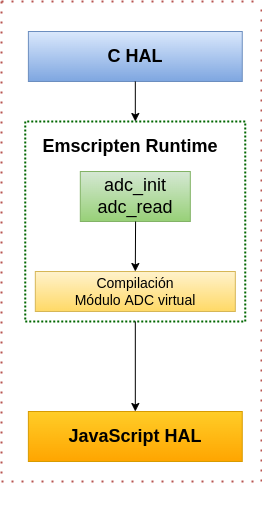
\includegraphics[scale=.52]{./Figures/adcEmscripten.png}
	\caption{Diagrama de bloques de \textit{C HAL} y \textit{JS HAL} para el módulo \textit{adc}.}
	\label{fig:adcEmscripten}
\end{figure}

En la capa \textit{JS UI}, se implementó la obtención de datos para los periféricos externos que interactúan con el \textit{adc}. 

Para el potenciómetro, los datos son establecidos por el usuario a través de la interfaz gráfica utilizando el componente HTML  \textit{input} de tipo \textit{range}. De esta manera, cuando el usuario desliza este componente dentro de un rango mínimo y máximo establecido (0 a 3.3V), se realiza el siguiente cálculo para obtener el valor del \textit{adc} correspondiente en un valor entero:

\begin{lstlisting}[caption={Cálculo del ADC para el potenciómetro.}]
  window.JSHal.gpio.write(self.dataPin.ADC, range.value/ 3.3 * 1023);
\end{lstlisting}

En consecuencia, los cálculos actualizados se muestran en la interfaz gráfica del emulador web emulando el comportamiento del conversor Analógico-Digital, que convierte de volteje a un número entero dependiendo de su resolución y voltaje de referencia. En el caso del \textit{ADC} del microcontroladore de la \textit{EDU-CIAA-NXP}, posee 10 bits de resolución (dando valores entre 0 y 1023) y 3.3V de voltaje de referencia.

Para la implementación del termistor NTC, se se reutiliza en la interfaz grafica un elemento gráfico (termómetro) para representar la temperatura en grados Celsius. A medida que el usuario ajusta el termómetro, la temperatura en kelvin se va actualizando en función de la temperatura en grados Celsius y, además, el valor del \textit{adc} se actualiza mediante la siguiente función:

\begin{lstlisting}[caption={Cálculo ADC del termistor NTC.}]
     ThermistorNTC.prototype.updateSampleADC= function(R_NTC) {
        let R_NTC_float = parseFloat(R_NTC);
        let R_10k_float = parseFloat(R_10k);
        let Vsupply_float = parseFloat(Vsupply);    
        let VoutT = (R_NTC_float * Vsupply_float) / (R_10k_float + R_NTC_float);
        Vout = parseFloat(VoutT.toFixed(2)); 

        this.sample = parseFloat((Vout * 1023.0 / Vsupply).toPrecision(4));
        console.log('this.sample ', this.sample);
        window.JSHal.gpio.write(this.dataPin.ADC, this.sample);     
    };
\end{lstlisting}

Esto permite convertir entre temperatura a voltaje y de allí a muestra leída por el ADC.

En el caso del \textit{AnalogStick} se implementó un componente web encargado de gestionar los movimientos y acciones en las interacciones con el usuario. Los datos de los movimientos de los ejes X e Y del \textit{AnalogStick} son obtenidos y se utilizan para realizar cálculos de voltajes en las respectivas resistencias de cada eje, así como también, para calcular el valor del \textit{adc}. A modo de referencia se muestra las cálculos para eleje X del \textit{AnalogStick}:

\begin{lstlisting}[caption={Cálculo de la resistencia del eje X y del ADC.}]
            var VRx = Joy.GetVRx();
            var voltage = (Math.floor(VRx/ 3.3 * 1023)* 3.3 / 1023.0).toFixed(2);
            joyVRx.textContent = voltage;
            joyADCx.textContent = Math.trunc(VRx/ 3.3 * 1023);
            window.JSHal.gpio.write(self.dataPin.ADCx, VRx/ 3.3 * 1023);
\end{lstlisting}

Luego, para cada periférico externo, el cálculo del \textit{adc} es envíado desde la capa \textit{JS UI} a la capa \textit{JS HAL}, como se esquematiza en la figura \ref{fig:uiADC}.

\begin{figure}[ht]
	\centering
	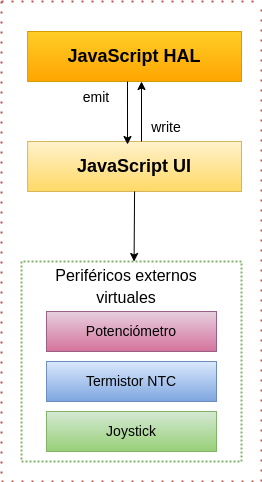
\includegraphics[scale=.57]{./Figures/uiADC.png}
	\caption{Diagrama de bloques con la interaccion entre las capas \textit{JS HAL} y \textit{JS UI}.}
	\label{fig:uiADC}
\end{figure}

\newpage
%-----------------------------------------
\subsection{\textit{\textbf{sapi\_tick}}}
\label{sec:sapi_tick}

En la tabla \ref{tab:sapiTick} se detallan las funciones del archivo de código fuente \texttt{sapi\_tick}.

\begin{table}[h]
	\centering
	\caption[Funciones \texttt{sapi\_tick}]{Funciones \texttt{sapi\_tick}}
	\begin{tabular}{p{0.20\linewidth} p{0.50\linewidth}  p{0.20\linewidth}}    
		\toprule
		\textbf{Función} 	 & \textbf{Parámetros} 		& \textbf{Tipo de retorno}  \\
		\midrule
		tickInit & tick\_t tickRateMSvalue 		&  bool\_t \\		
		tickRead	 & void				&  tick\_t \\
		tickWrite	 & tick\_t ticks 				& void \\
		tickCallbackSet	 & callBackFuncPtr\_t tickCallback, void* tickCallbackParams				&  bool\_t \\
		tickPowerSet & bool\_t power 		&  void \\	
		\bottomrule
		\hline
	\end{tabular}
	\label{tab:sapiTick}
\end{table}

Para emular a nivel de API, se tuvo como objetivo replicar el comportamiento de la función \texttt{tickInit}, la cual se encarga de la inicialización y configuración de la interrupción del temporizador \texttt{SysTick\_Config} en la placa física. Sin embargo, al realizar la emulación en la plataforma web, esta función no se encuentra disponible de forma nativa. Por lo tanto, fue necesario emular su comportamiento y proporcionar una alternativa compatible.

Para emular la funcionalidad de \texttt{SysTick\_Config}, se utilizó la capa de emulación correspondiente a \textit{C HAL}. Esta capa de emulación permitió ejecutar código \textit{JavaScript} en el contexto de \textit{Emscripten}, lo que posibilitó replicar el comportamiento del temporizador \textit{SysTick}. 

Una vez habilitada la interrupción del temporizador, se realiza una invocación periódica a la función \texttt{tickerCallback}, que tiene la misma implementación que en \texttt{sapi\_tick} de la biblioteca \textit{\textbf{sAPI}} del proyecto CIAA. La función \newline \texttt{tickerCallback} realiza las siguientes acciones: incrementa el contador de ticks y, si el puntero \texttt{tickHookFunction} no es nulo, ejecuta la función establecida como \textit{callback} mediante la función de \textit{\textbf{sAPI}} \texttt{tickCallbackSet()}, pasando los parámetros \texttt{callBackFuncParams}. En consecuencia, esto permite la ejecución de tareas específicas programadas por el usuario en cada interrupción del temporizador periódico.

Para emular el comportamiento de la interrupción del temporizador \textit{SysTick} y proporcionar la invocación periódica a la función \texttt{tickerCallback} de \textit{sapi\_tick}, se utilizó la macro \texttt{EMSCRIPTEN\_KEEPALIVE} de \textit{Emscripten}, que le dice al compilador de \textit{Emscripten} que conserve la función marcada con esta macro en el código compilado, incluso si no es accedida desde el código \textit{JavaScript} del lado del cliente.

Es decir, cuando la función marcada con la macro \texttt{EMSCRIPTEN\_KEEPALIVE} sea invocada desde la capa \textit{JavaScript HAL}, llamará a la función \texttt{tickerCallback} de la biblioteca \textit{C} y la ejecutará. En la figura \ref{fig:tickerCallback} se muestra el funcionamiento de \texttt{EMSCRIPTEN\_KEEPALIVE}. 

\begin{figure}[ht]
	\centering
	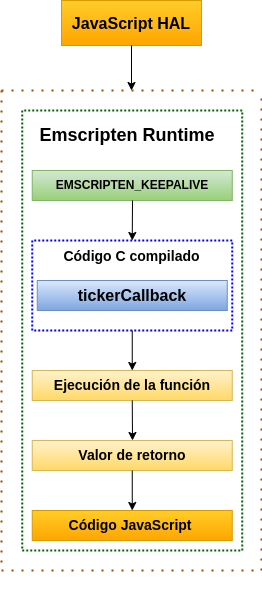
\includegraphics[scale=.46]{./Figures/tickerCallback.png}
	\caption{Diagrama de bloques \texttt{EMSCRIPTEN\_KEEPALIVE}.}
	\label{fig:tickerCallback}
\end{figure}

Para lograr la interacción con la capa de emulación \textit{C HAL}, y realizar la invocación periódica a la función que usa la macro \texttt{EMSCRIPTEN\_KEEPALIVE} de \textit{Emscripten} se configuró en esta capa de desarrollo un temporizador de \textit{JavaScript}.

Además, dentro del temporizador, se utilizó la función \texttt{ccall} de \textit{Emscripten}, que permite invocar a la funcion \texttt{tickerCallback} desde el código \textit{C} compilado con \textit{Emscripten}. 

A continuacion, se muestra en la figura  \ref{fig:ccall} el funcionamiento de \texttt{ccall}. 

\begin{figure}[ht]
	\centering
	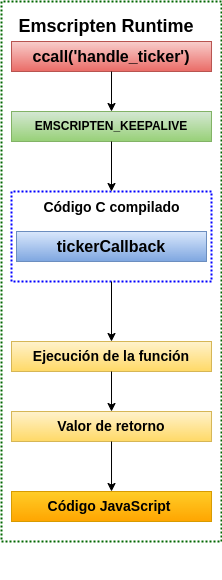
\includegraphics[scale=.46]{./Figures/ccall.png}
	\caption{Diagrama de bloques de la función \textit{ccall}.}
	\label{fig:ccall}
\end{figure}

Sin embargo, debido a la naturaleza asíncrona de \textit{JavaScript} y al uso de la función \texttt{ccall}, la función no mantiene el contexto entre las ejecuciones del temporizador. En consecuencia, cada vez que se reinicia el temporizador y se ejecuta la función  \texttt{tickerCallback}, la tarea específica programada por el usuario comienza desde el principio en lugar de continuar desde el punto donde quedó anteriormente. 

En el capítulo 4 se detallarán las diferencias encontradas al realizar las pruebas entre la placa y el emulador utilizando estas funciones.

\newpage
%-----------------------------------------
\subsection{\textit{\textbf{sapi\_delay}}}

La tabla \ref{tab:sapiDelay} expone las funciones del archivo de código fuente \texttt{sapi\_delay}.

\begin{table}[h]
	\centering
	\caption[Funciones \texttt{sapi\_delay}]{Funciones \texttt{sapi\_delay}}
	\begin{tabular}{p{0.30\linewidth} p{0.40\linewidth}  p{0.20\linewidth}}    
		\toprule
		\textbf{Función} 	 & \textbf{Parámetros} 		& \textbf{Tipo de retorno}  \\
		\midrule
		delayInaccurateMs & tick\_t delay\_ms 		&  void \\		
		delayInaccurateUs	 & tick\_t delay\_us			&  void \\
		delayInaccurateNs	 & tick\_t delay\_ns				& void \\
		delay	 & tick\_t duration\_ms				&  void \\
		delayInit & delay\_t * delay, tick\_t duration 		&  void \\
		delayRead & delay\_t * delay 		&  bool\_t \\
		delayWrite & delay\_t * delay, tick\_t duration 		&  void \\	
		\bottomrule
		\hline
	\end{tabular}
	\label{tab:sapiDelay}
\end{table}

La función \texttt{delay} en la biblioteca \textit{\textbf{sAPI}} del proyecto CIAA crea una pausa en la ejecución del programa durante el tiempo especificado en \texttt{duration\_ms} implementando un bucle de espera. Este bucle bloqueante se ejecutará mientras la diferencia de tiempo entre \texttt{tickRead()} y startTime(inicio actual de \texttt{tickRead()} sea menor que \texttt{duration\_ms/ tickRateMS}.

Este comortamiento cae en las limitaciones de \textit{Arm Mbed OS Simulator}, presentadas en la sección \ref{sec:Análisis de los emuladores revisados}, causando que la ejecución de la plataforma web se bloquee o congele, debido a que es como si se ejecutase un \textit{while(1)}. Por esta razón, se decide utilizar en su lugar las funciones nativas de \textit{Emscripten} en la capa de emulación \textit{C HAL}. En consecuencia, se aprovecho su eficiencia y precisión.

Para emular las funciones de espera de la biblioteca \textit{C} se utiliza la función \newline \texttt{emscripten\_sleep}, que usa funciones asincrónicas internas de \textit{Emscripten} para realizar pausas. Por lo tanto, permite al navegador atender otros eventos mientras el programa se encuentra en espera. De esta manera, evita el bloqueo de la ejecución del resto del código y también, que la página no responda. Además, proporciona pausas precisas, debido a que, \textit{Emscripten} utiliza las capacidades de temporización del navegador para garantizar que el tiempo indicado sea realizado. La figura \ref{fig:emscriptenDelay} representa el funcionamiento de  \texttt{emscripten\_sleep}. 

\begin{figure}[ht]
	\centering
	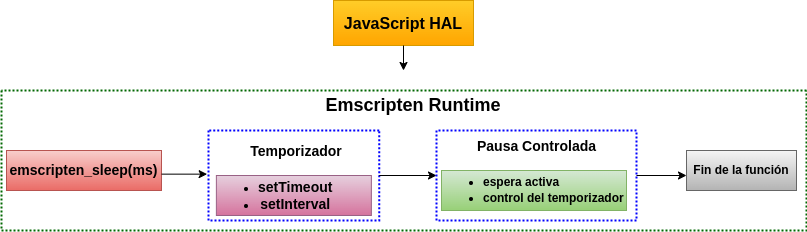
\includegraphics[scale=.48]{./Figures/emscriptenDelay.png}
	\caption{Diagrama de bloques \texttt{emscripten\_sleep.}}
	\label{fig:emscriptenDelay}
\end{figure}

\newpage
%------------------------------------------
\subsection{\textit{\textbf{sapi\_dht11}}}

Para emular drivers de periféricos externos de la biblioteca \textit{\textbf{sAPI}}, se continuó con la misma lógica de programación utilizada para interactuar con los periféricos internos. Estos se mapean las funcionalidades ofrecidas por la biblioteca \textit{\textbf{sAPI}} a la plataforma web. En la siguiente tabla \ref{tab:sapiDht11} se describen las funciones presentes.

\begin{table}[h]
	\centering
	\caption[Funciones \texttt{sapi\_dht11}]{Funciones \texttt{sapi\_dht11}}
	\begin{tabular}{p{0.20\linewidth} p{0.50\linewidth}  p{0.20\linewidth}}    
		\toprule
		\textbf{Función} 	 & \textbf{Parámetros} 		& \textbf{Tipo de retorno}  \\
		\midrule
		dht11Init & int32\_t gpio		&  void \\		
		dht11Read	 & float *phum, float *ptemp	&  bool\_t \\
		\bottomrule
		\hline
	\end{tabular}
	\label{tab:sapiDht11}
\end{table}

En esta primera versión de la plataforma web, no se ofrece la capacidad gráfica de realizar las conexiones mediante cables virtuales entre la placa y los periféricos externos. Simplemente se muestran indicados los pines que el usuario debe elegir, para configurar a qué pin se conecta cada pin del sensor de humedad y temperatura \textit{DHT11}. Estas conexiones luego serán verificadas en la capa de \textit{JS UI}.

En la capa \textit{JS UI} se centra principalmente el trabajo de emular el envío de los datos de temperatura y humedad del sensor \textit{DHT11} a la placa de desarrollo.
Entonces, en la capa de abstracción de datos \textit{C HAL} se implementa la lectura de los datos provenientes de la capa \textit{JS HAL} al usar la macro \texttt{EM\_ASM\_INT} de \textit{Emscripten}, que se presenta mediante un diagrama en bloques en la figura \ref{fig:dht11Emscripten}.

\begin{figure}[ht]
	\centering
	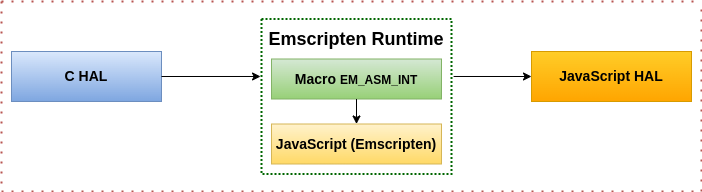
\includegraphics[scale=.55]{./Figures/dht11Emscripten.png}
	\caption{Diagrama de bloques de la macro \texttt{EM\_ASM\_INT}.}
	\label{fig:dht11Emscripten}
\end{figure}

La capa \textit{JS HAL} recibe los datos enviados desde \textit{JS UI} y los transmite a la capa \textit{C HAL}. La generación de los datos  emulados de temperatura y humedad, se realiza en \textit{JS UI} a través de dos opciones elegidas por el usuario:
 
 \begin{itemize}
	\item Obtener los datos de temperatura y humedad local conectándose a una central meteorológica a través de la geolocalización del navegador del usuario. Sin embargo, si el servidor donde se encuentra desplegada la plataforma web no puede acceder al servicio de geolocalización del navegador por motivos de seguridad, o el usuario no permite el acceso, entonces se realizará la consulta a la central meteorológica utilizando la ubicación predeterminada de la ciudad de Buenos Aires. Acto seguido se actualizará la interfaz gráfica con los datos de temperatura y humedad.
	
	\item Generar los datos manualmente haciendo \textit{click} en la interfaz gráfica que representa a la temperatura y humedad. De esta manera, el usuario puede generar los datos según su elección.
\end{itemize}

En la figura \ref{fig:uiDht11} se muestra el diagrama de bloques de la capa de interfaz de usuario \textit{JavaScript UI} con las dos opciones de usuario.

\begin{figure}[ht]
	\centering
	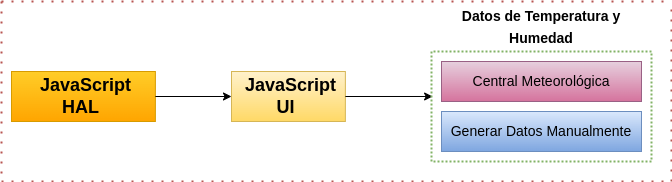
\includegraphics[scale=.53]{./Figures/uiDht11.png}
	\caption{Diagrama de bloques de la capa \textit{JavaScript UI} con las dos opciones para el usuario.}
	\label{fig:uiDht11}
\end{figure}

%----------------------------------------------------------------------------------------
\section{\textit{freeRTOS}}
\label{sec:freeRTOS}
%----------------------------------------------------------------------------------------

Para emular la funcionalidad de las tareas de \textit{freeRTOS} en el contexto del emulador web, se utilizó la biblioteca de eventos de \textit{mbed}. Entonces, para las funciones \texttt{xTaskCreate} y \texttt{xTaskCreateStatic}, se programaron funciones periódicas utilizando las siguientes funciones de la biblioteca de \textit{Mbed events}: 

 \begin{itemize}
	\item \texttt{int equeue\_create}:  crea una cola de eventos, configura e inicializa los recursos de plataforma necesarios, como semáforos y mutexes.
	
	\item \texttt{int equeue\_call\_every}:  se utiliza para crear un evento periódico en la cola de eventos equeue, programando llamadas repetidas a una función en intervalos regulares.
	
	\item \texttt{int equeue\_post}: permite publicar un evento en la cola de eventos equeue, estableciendo el tiempo y estableciendo el evento en la cola para su posterior procesamiento.
	
	\item \texttt{void equeue\_dispatch}: se encarga de despachar los eventos en la cola de eventos equeue de manera continua, verificando los tiempo y realizando acciones específicas según la configuración.

	\item \texttt{void equeue\_destroy}: permite liberar y limpiar todos los recursos asociados a una cola de eventos, libera los mutexes, semáforos y memoria asignada.
\end{itemize}

Estas funciones permiten ejecutar tareas periódicas en intervalos de tiempo regulares, lo que proporciona una aproximación simplificada a la funcionalidad de tareas en el emulador web. Aunque esta solución no ofrece todas las características de un sistema operativo de tiempo real completo como \textit{freeRTOS}, fue adecuada para emular el funcionamiento de programas de usuario simples.

Es importante destacar que la implementación de tareas en el emulador web tiene una limitación significativa. Debido a que solo puede ejecutar un subproceso (hilo de ejecución) a la vez, no es posible que se ejecuten tareas simultáneas. Esto significa que, a diferencia del sistema operativo de tiempo real \textit{freeRTOS}, donde se pueden crear múltiples tareas que se ejecutan de manera concurrente, en el emulador web solo es posible ejecutar una sola tarea. Por lo tanto, esta solución es adecuada para programas de usuario simples que no requieran multitarea.

La tabla \ref{tab:ConceptosRTOS} expone la comparación entre funcionalidades presentes en \textit{freeRTOS} y las implementadas en \textit{EmuCIAA.}.

\begin{table}[h]
\centering
\caption[Comparación entre funcionalidades de \textit{freeRTOS} que se cumplen en el emulador.]{Comparación entre funcionalidades de \textit{freeRTOS} y las implementadas en \textit{EmuCIAA.}}
\begin{tabular}{p{0.45\linewidth} p{0.15\linewidth}  p{0.15\linewidth}}
\toprule
\textbf{Funcionalidad} 
& \textbf{\textit{freeRTOS}}
& \textbf{Emulador}
\\
\midrule
Multitareas & Si & No  \\
Funciones de espera &  Si & Si \\
Cambio de contexto &  Si & Si \\
Tarea de procesamiento continuo &  Si & Si \\
Manejo de prioridades & Si & No  \\
\bottomrule
\hline
\end{tabular}
\label{tab:ConceptosRTOS}
\end{table}

En esta primera versión del emulador, no se han incluido el manejo de multitareas y de prioridades presentes en \textit{freeRTOS}.

%----------------------------------------------------------------------------------------
\section{Comparación de periféricos implementados}
%----------------------------------------------------------------------------------------

La tabla \ref{tab:perifericosInternosMBED} expone los  periféricos internos implementados actualmente en \textit{Mbed OS Simulator} y los implementados en \textit{EmuCIAA}.

\begin{table}[htbp]
\centering
\caption[Periféricos internos implementados]{Comparación de periféricos internos implementados en \textit{Mbed OS Simulator} y  \textit{EmuCIAA}}
\begin{tabular}{p{0.24\linewidth} p{0.14\linewidth}  p{0.14\linewidth}  p{0.14\linewidth}}
\toprule
\textbf{Periféricos} 
& \textbf{MbeOS Sim}
& \textbf{EmuCIAA}
\\
\midrule
GPIO & Si & Si  \\
UART & Si & Si \\
BUTTON & SI & Si \\
ADC & Si & Si \\
DAC & Si & No \\
PWM & Si & No \\ 
RTC & No & Si \\ 
Systick & No & Si \\ 
\bottomrule
\hline
\end{tabular}
\label{tab:perifericosInternosMBED}
\end{table}

En la tabla \ref{tab:perifericosExternosMBED} se comparan los periféricos externos implementados actualmente en \textit{Mbed Simulator} con los implementados en \textit{EmuCIAA},

\hfill \break
\hfill \break
\hfill \break
\hfill \break
\hfill \break
\hfill \break
\hfill \break
\hfill \break
\hfill \break
\hfill \break
\hfill \break

\begin{table}[htbp]
\centering
\caption[Periféricos externos]{Comparación de periféricos externos implementados en \textit{Mbed OS Simulator} y  \textit{EmuCIAA}}
\begin{tabular}{p{0.24\linewidth} p{0.14\linewidth}  p{0.14\linewidth}  p{0.14\linewidth}}
\toprule
\textbf{Periféricos} 
& \textbf{MbeOS Sim}
& \textbf{EmuCIAA}
\\
\midrule
LED Rojo & Si & Si \\
LED Azul & Si & Si \\
LED Amarillo & Si & Si \\
LED Blanco & Si & Si \\
Potenciómetro & No & Si \\
AnalogStick & No & Si \\
Termistor NTC & Si & Si \\
DHT11 & Si & Si  \\
SHT31 & Si & No \\
LCD C12832 & Si & No  \\
ST7789H2 & Si & No \\
LCD HDD44780 & No & Si  \\
GLCD ST7920 & No & Si  \\
\bottomrule
\hline
\end{tabular}
\label{tab:perifericosExternosMBED}
\end{table}

Finalmente, se compara el aspecto visual entre ambas paltaformas en las figuras \ref{fig:perifericosMbed}, para \textit{Mbed OS Simulator}, y \ref{fig:perifericosCIAA} para \textit{EmuCIAA}. De estas figuras se observa como para el desarrollo de \textit{EmuCIAA} se tuvo especial cuidado para emular los componentes externos de la forma más fiel posible a la relaidad y mostrar las conexiones de los pines de forma didáctica.

\begin{figure}[ht]
	\centering
	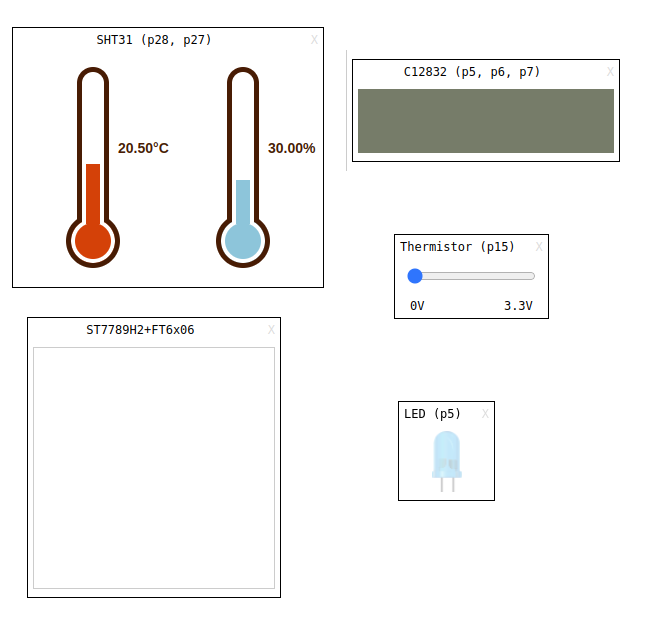
\includegraphics[scale=.85]{./Figures/perifericosMBED.png}
	\caption{Periféricos externos de \textit{Arm Mbed OS Simulator}.}
	\label{fig:perifericosMbed}
\end{figure}

\begin{figure}[p]
	\centering
	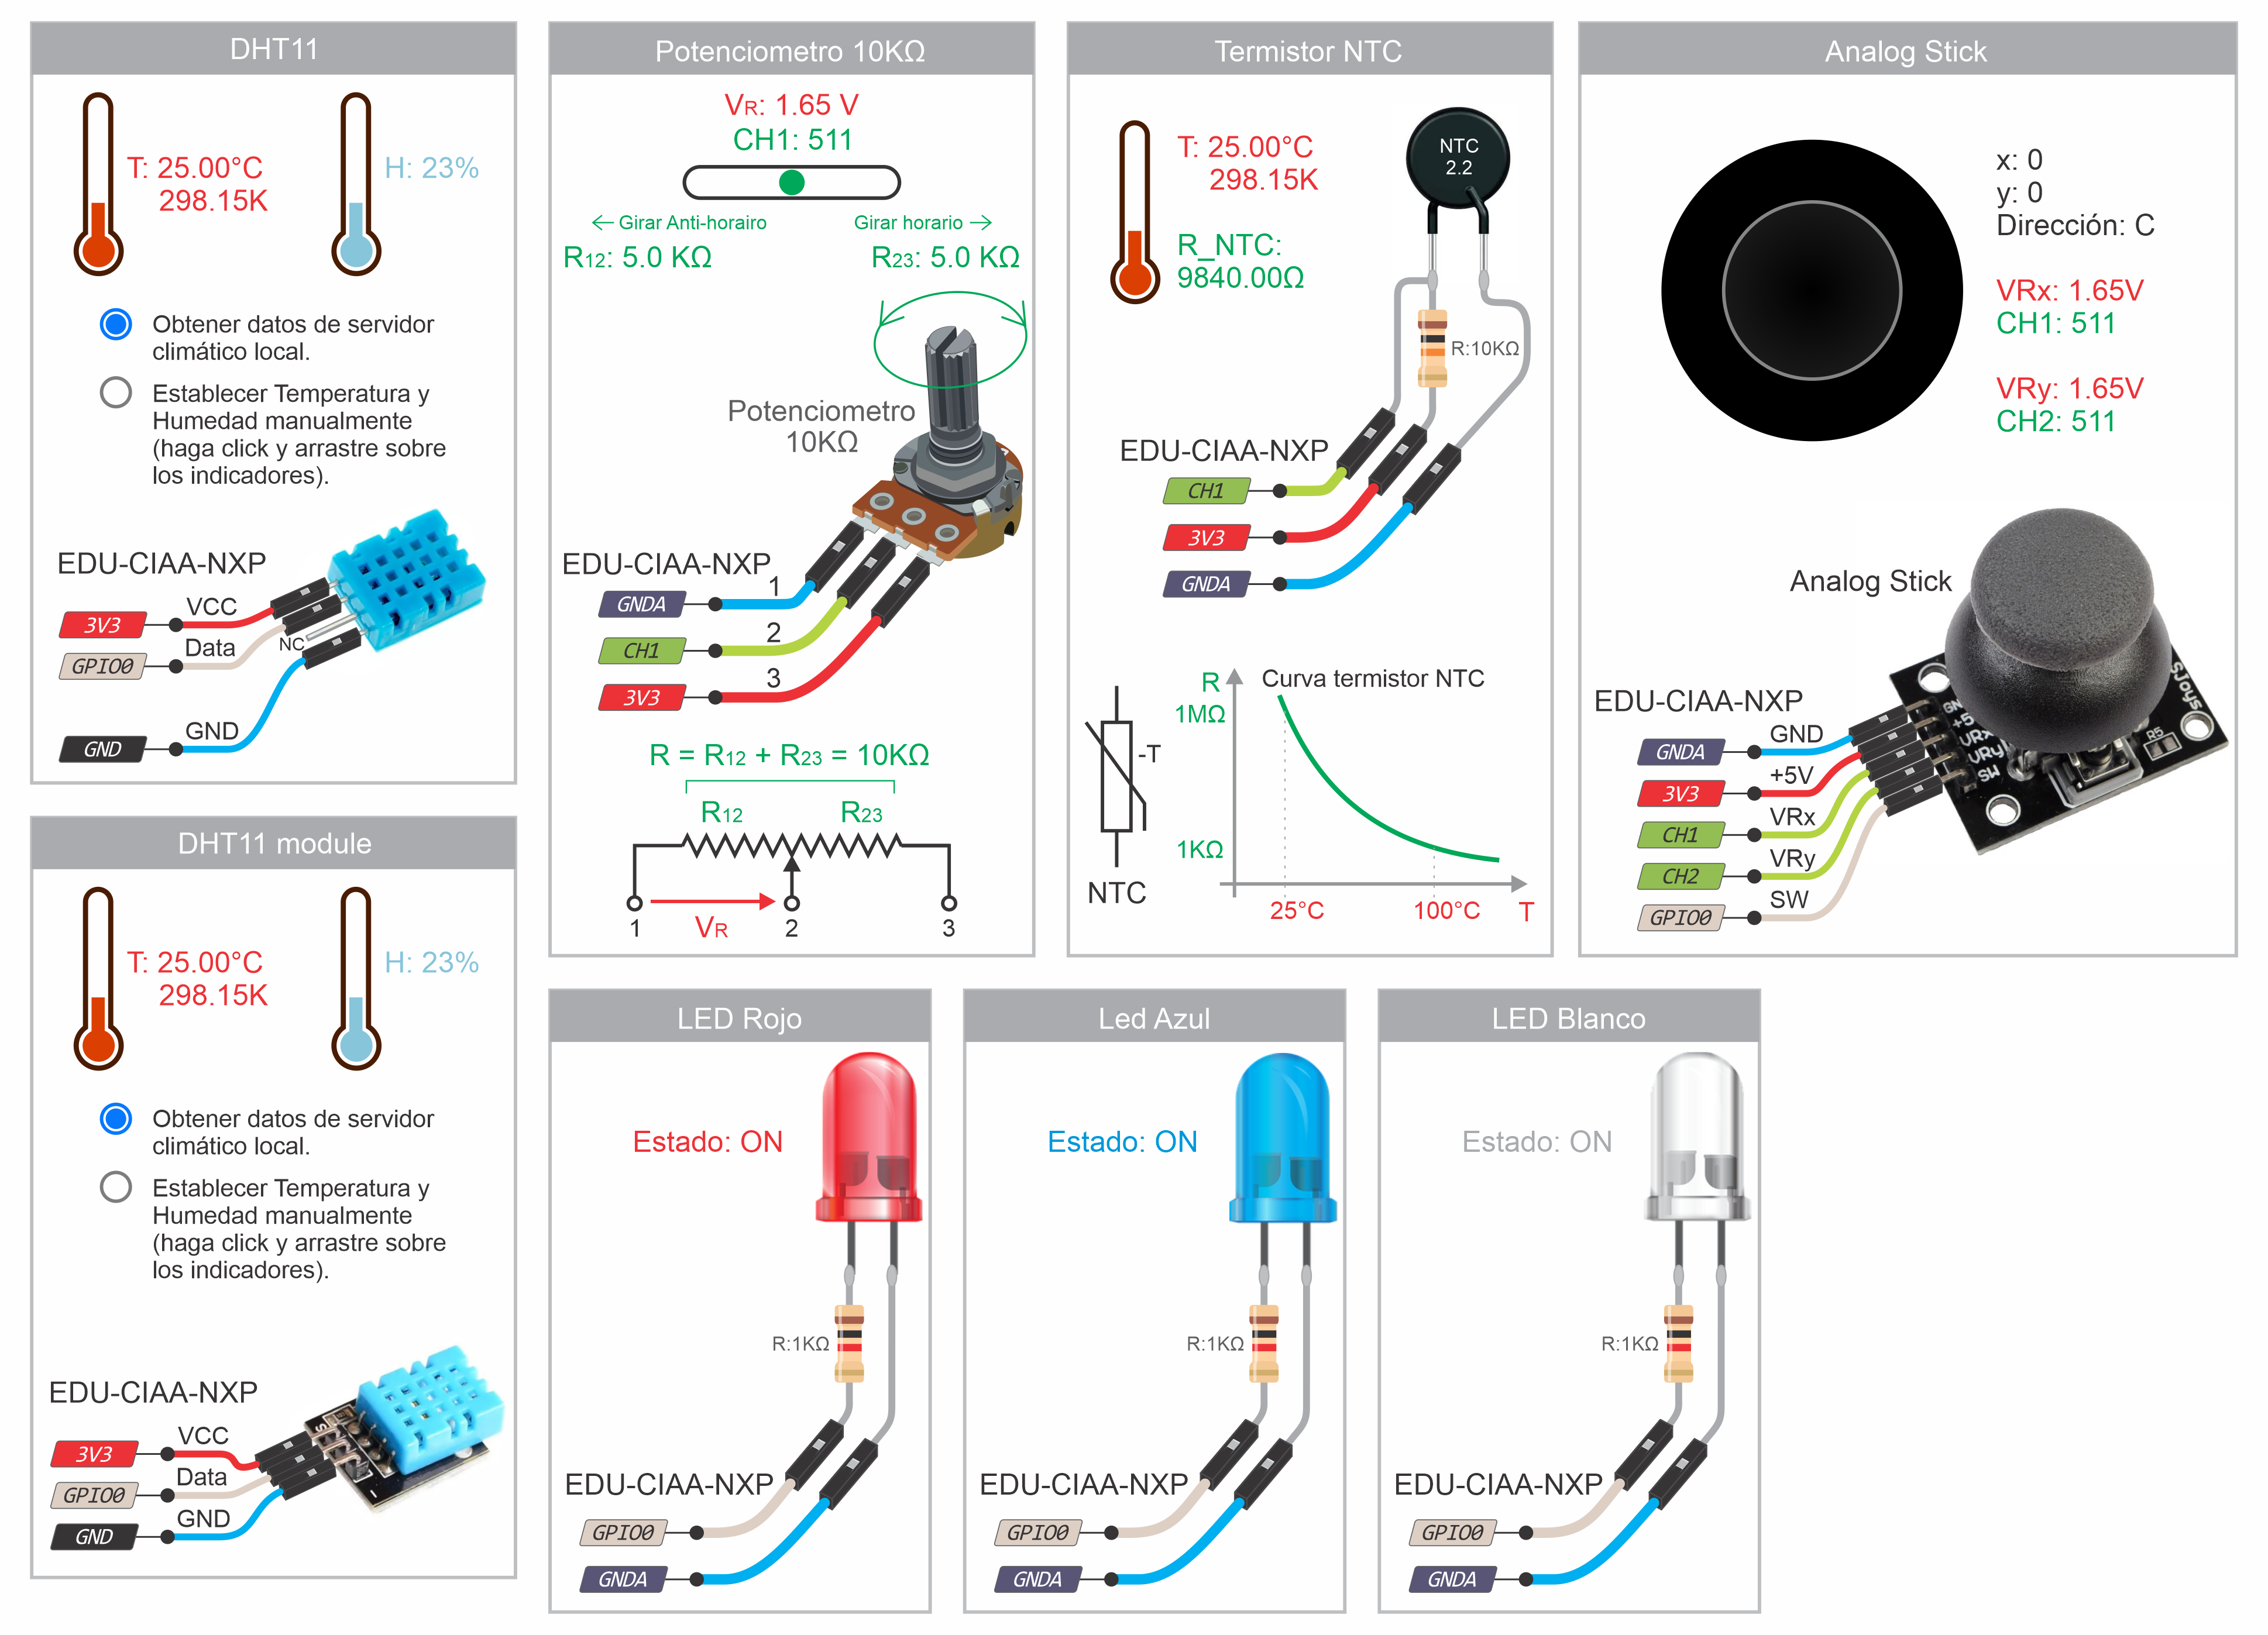
\includegraphics[scale=.58]{./Figures/perifericosCIAA.png}
	\caption{Periféricos externos del emulador web EDU-CIAA.}
	\label{fig:perifericosCIAA}
\end{figure}

\newpage
%----------------------------------------------------------------------------------------
\section{Ejemplos incluidos}
%----------------------------------------------------------------------------------------

Se incluyen en la plataforma los sigueintes ejemplos de programas, los cuales se ordenaron cuidadosamente para permitir que se pueda ir aprendiendo de forma incremental el uso de varios periféricos y técnicas de programación de Sistemas Embebidos:

\begin{itemize}

\item \textbf{GPIO}
    \begin{itemize}
    \item blinky
    \item semaphore
    \item blinky\_switch
    \item switches\_leds
    \item led\_sequences
    \end{itemize}

\item \textbf{UART}
    \begin{itemize}
    \item serial\_output
    \end{itemize}

\item \textbf{RTC}
    \begin{itemize}
    \item rtc\_uart
    \item rtc\_prinf
    \end{itemize}

\item \textbf{ADC}
    \begin{itemize}
    \item portentiometer
    \item ntc\_thermistor
    \item analog\_stick
    \end{itemize}
\item \textbf{Tick}
    \begin{itemize}
    \item tick\_callback
    \end{itemize}

\item \textbf{Sensors}
    \begin{itemize}
    \item dht11\_temp\_humidity
    \end{itemize}

\item \textbf{Displays}
    \begin{itemize}
    \item lcd\_hd44780\_c20x4\_gpios
    \item lcd\_hd44780\_custom\_chars
    \item glcd\_st7920\_c16x4
    \item glcd\_st7920\_g128x64 
    \end{itemize}

\item \textbf{Non-bloking code}
    \begin{itemize}
    \item little\_delay
    \item tick\_counter
    \item non\_blocking\_delay
    \end{itemize}

\item \textbf{FSM}
    \begin{itemize}
    \item semaphore
    \item debounce
    \item button
    \end{itemize}

\item \textbf{RTOS cooperative}
    \begin{itemize}
    \item scheduler
    \item scheduler\_bgfg
    \end{itemize}

\item \textbf{RTOS SEOS Pont}
    \begin{itemize}
    \item pont\_blinky
    \item pont\_tasks\_parameters
    \item pont\_modular\_tasks
    \item pont\_uart\_clock
    \end{itemize}

\item \textbf{RTOS FreeRTOS}
    \begin{itemize}
    \item freertos\_blinky\_dynamic\_men
    \item freertos\_blinky\_static\_men
    \end{itemize}

\end{itemize}

La mayoría de estos ejemplos fueron seleccionarion de \textit{firmware\_v3}. Los nuevos programas realizados para \textit{EmuCIAA} son:

\begin{itemize}
    \item serial\_output
    \item portentiometer
    \item ntc\_thermistor
    \item analog\_stick
    \item glcd\_st7920\_c16x4
    \item glcd\_st7920\_g128x64 
\end{itemize}

%----------------------------------------------------------------------------------------
\section{Despliegue en un servidor web}
%----------------------------------------------------------------------------------------

Para hacer público \textit{EmuCIAA} en un servidor web, se realizó el proceso de despliegue en el servidor de \textit{DigitalOcean} mediante los siguientes pasos:

\begin{itemize}
	\item Crear una cuenta: que implica registrar una cuenta en la plataforma. Iniciar sesión y crear un \textit{droplet}, que es un servidor virtual. Luego, se instala el sistema operativo, en este caso, \textit{Ubuntu}, y se configura la región geográfica donde se ubicaría el servidor y la cantidad de RAM a utilizar.
	
	\item Acceso al servidor: se obtiene la dirección IP pública y la clave \textit{SSH} para acceder al servidor.
	
	\item Configuración: implica instalar las herramientas, como \textit{Mbed CLI} y \textit{Emscripten}, y también, los servicios necesarios, como los entornos de ejecución de \textit{Node.js} y \textit{Python}. Además, se realizan las configuraciones de las reglas de \textit{firewall}.

	\item Copiar la plataforma web al servidor: se utiliza \textit{GitHub} para clonar el repositorio en el servidor. El código del presente trabajo, se encuentra en el repositorio de GitHub \citep{repositorioEmulador}.
	
	\item Iniciar el emulador web: se utiliza la herramienta \textit{TMUX} para mantener la sesión y la ventana de la terminal donde se ejecuta la aplicación de forma persistente, incluso cuando se cierra la conexión \textit{SSH}. El presente trabajo, se encuentra actualmente ejecutandose en la \textit{URL}: \url{http://134.209.168.175:7900}.
\end{itemize}